\subsubsection{Glyptemys --- Sculptured Turtles (Wood and Bog Turtle)}
\begin{center}
\begin{longtabu} to \textwidth {| | p{3.5cm} | X | |}

	\hline
	Taxonomy/Ancestry &
	subfamily Emydinae. 2 N. American species, bog and wood turtles. formerly considered members of \emph{Clemmys}. 50 chromosome karyotypes.
	
	During the last post-Pleistocene ice age, Glyptemys turtles were forced south by encroaching glaciers from the north. After glaciation, some turtle colonies relocated to their original northern range, while others continued to live in the new, southern range. Some fossil remains from the Rancholabrean period (300,000 to 11,000 years BP) have been found in Georgia and Tennessee, areas farther south than the turtles' current range.
	
	\begin{center} \includegraphics[scale=0.5]{testudines/emydidae/glyptemys/tax} \end{center}
	 \\
	\hline
	Size & 
	Glyptemys turtles are small to medium in size: the bog turtle males grow to be 9.4 cm (3.7 in) and females 8.9 cm (3.5 in) while wood turtles of either gender reach 14 to 20 cm (5.5 to 7.9 in) in length. Bog turtles weigh 110 g (3.9 oz) and wood turtles average 1 kg (2.2 lb) at maturity.
	\\
	\hline
	Color &
	bog has small, bright blotches on each side of the neck. wood has dark grey to black head w/ bright orange coloration on ventral surfaces.
	 \\
	\hline
	Anatomy &
	
	 \\
	\hline
	Dimorphism & 
	
	\\
	\hline
	Behavior & 
	These turtles are diurnal and become active in the early morning.During extremely cold days, they each may spend time under water, while the bog has been known to also seek dense underbrush or mud in which to bury itself. Excessively hot days sometimes causes these turtles to estivate.
	\\
	\hline
	Habitat & 
	These turtles are semiaquatic and are commonly found in bogs, fens, and small streams which have soft yet compacted, sandy bottoms.
	\\
	\hline
	Distribution & 
	Glyptemys turtles are endemic to eastern North America. Their collective range extends from Nova Scotia south to Georgia and from Nova Scotia west to Minnesota.  
	\\
	\hline
	Feeding Ecology & 
	 feed on insects, plant matter, small invertebrates, and carrion.
	\\
	\hline
	Reproductive Biology & 
	
	\\
	\hline
	Ecological Role &
	
	\\
	\hline
	Conservation Status & 
	Both species are protected throughout their ranges. The bog turtle is considered endangered, while the wood turtle is labeled as vulnerable, a less dire rating.
	\\
	\hline
\end{longtabu}
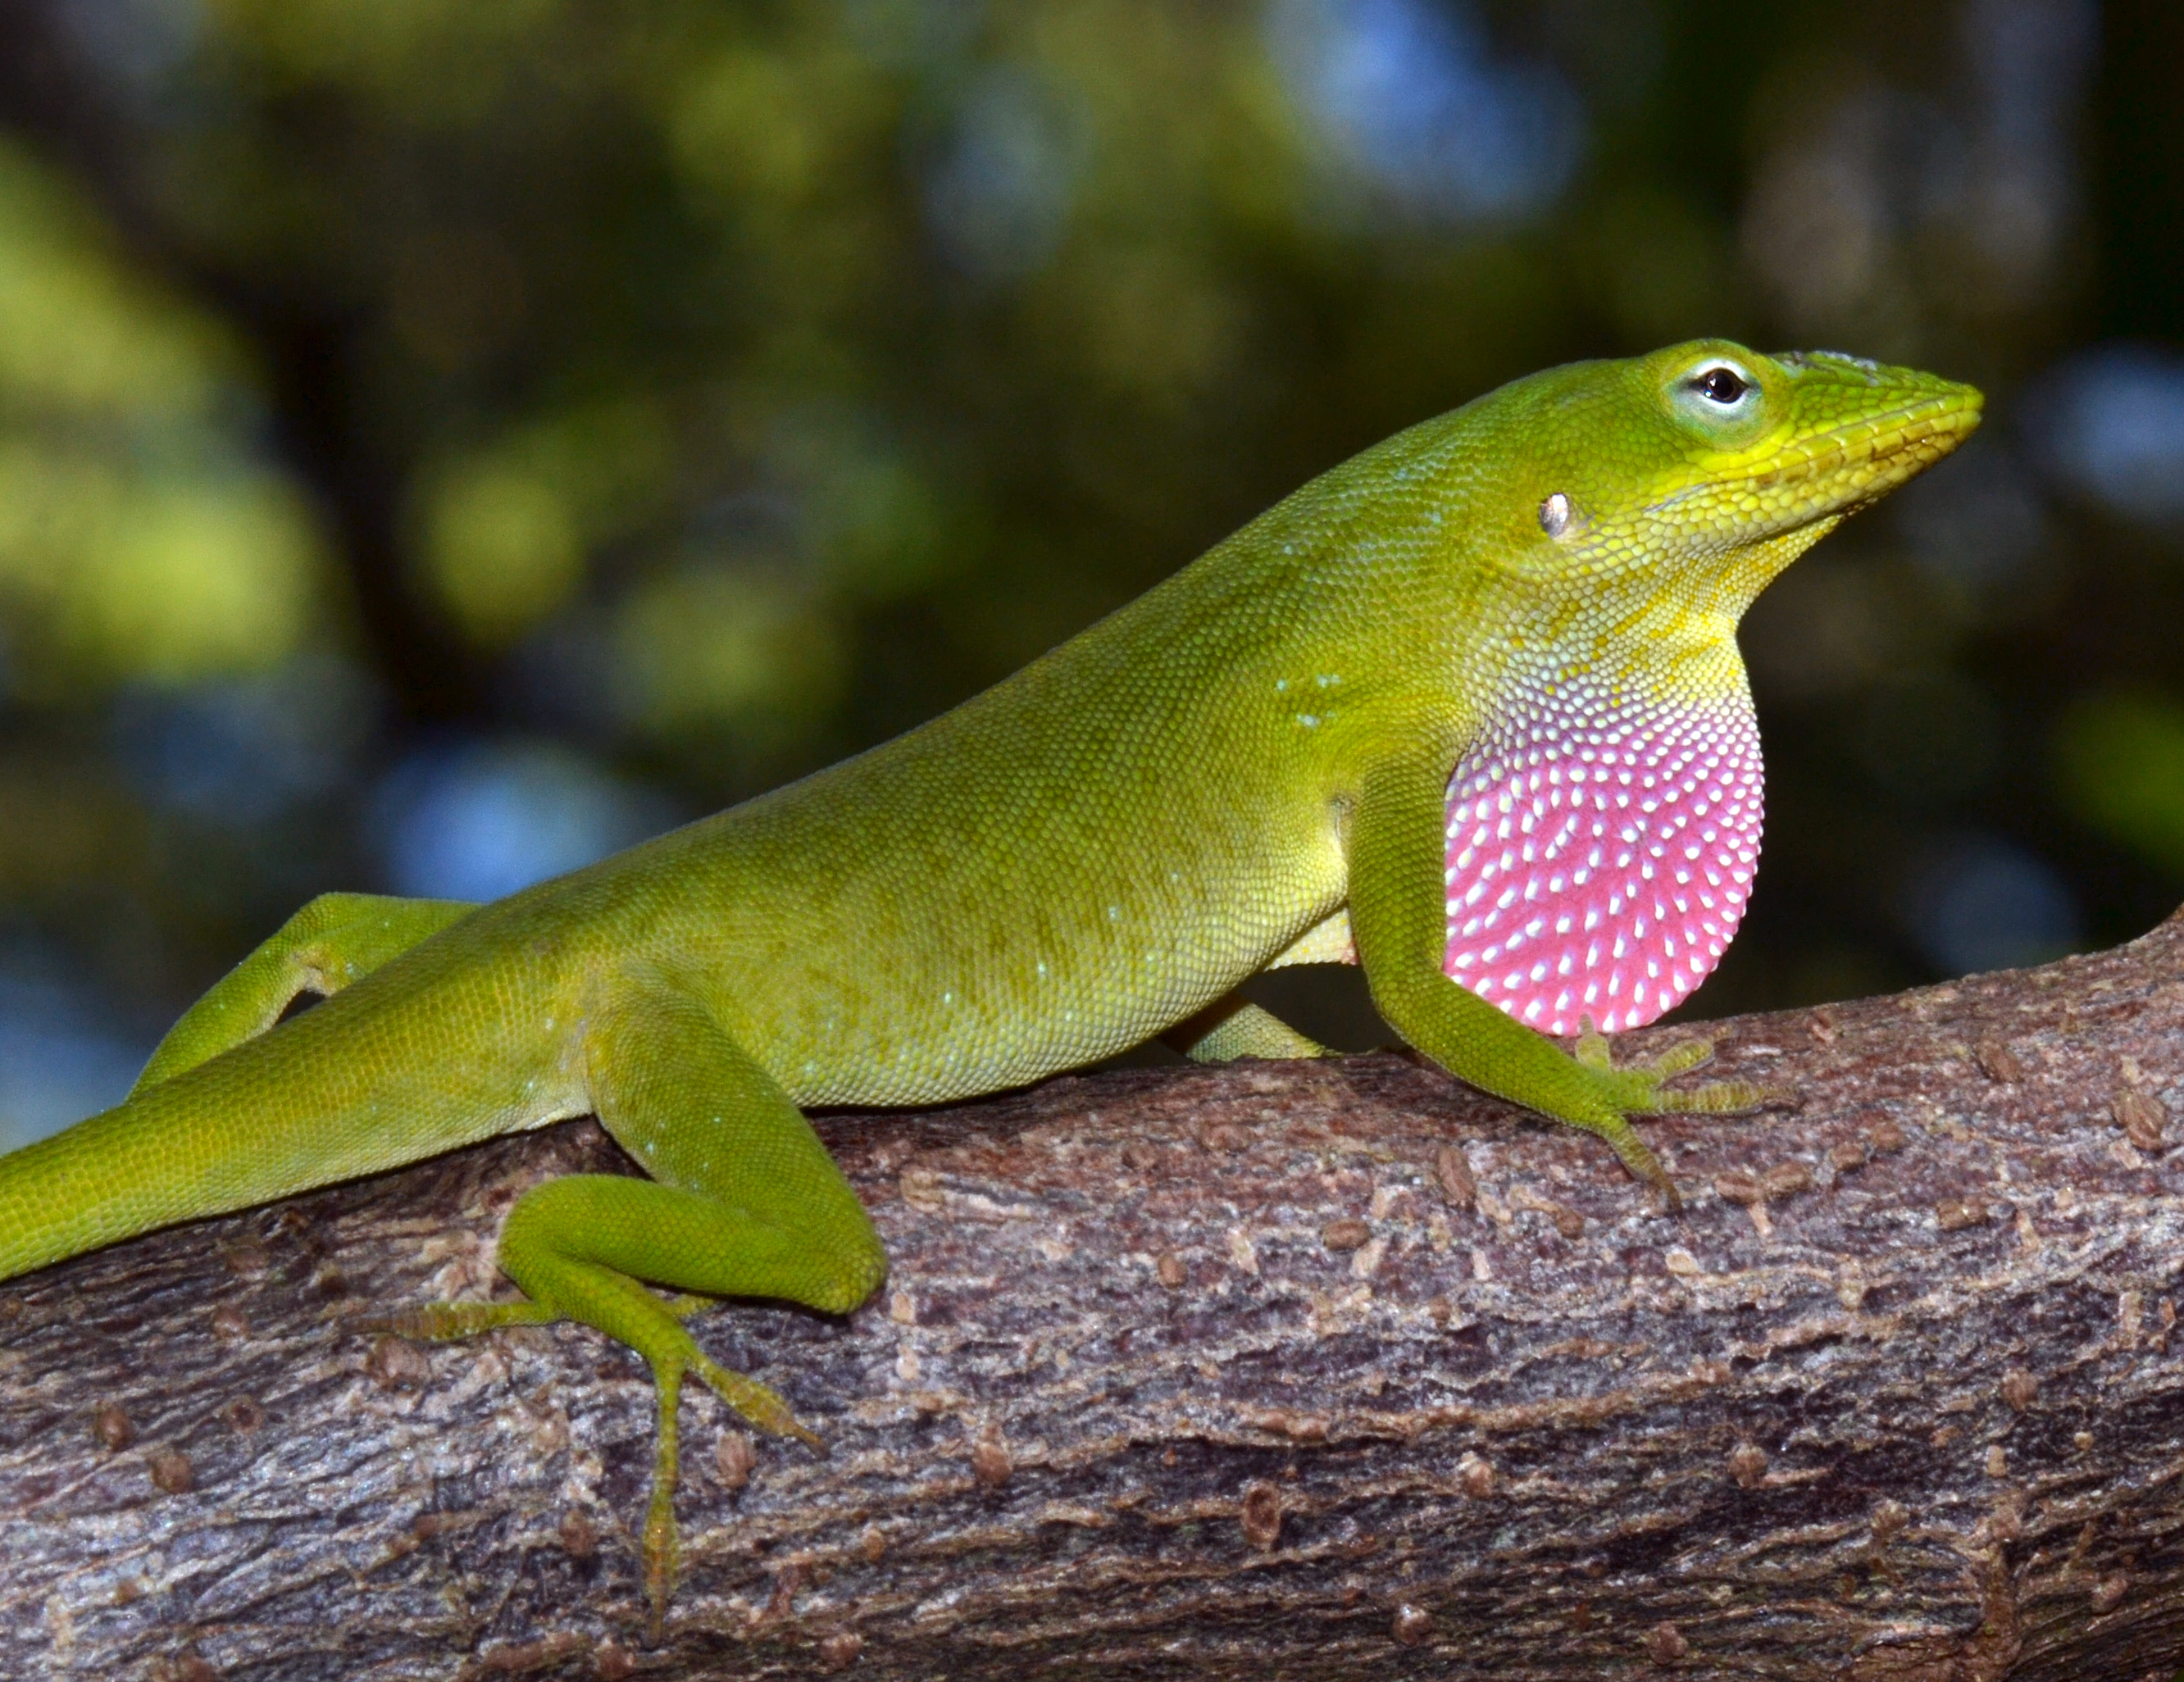
\includegraphics[scale=0.5]{testudines/emydidae/glyptemys/1}
\includegraphics[scale=0.15]{testudines/emydidae/glyptemys/2}
\end{center}